\documentclass{article}
% translate with >> pdflatex -shell-escape <file>

% This file is an extract of the PGFPLOTS manual, copyright by Christian Feuersaenger.
% 
% Feel free to use it as long as you cite the pgfplots manual properly.
%
% See
%   http://pgfplots.sourceforge.net/pgfplots.pdf
% for the complete manual.
%
% Any required input files (for <plot table> or <plot file> or the table package) can be downloaded
% at
% http://www.ctan.org/tex-archive/graphics/pgf/contrib/pgfplots/doc/latex/
% and
% http://www.ctan.org/tex-archive/graphics/pgf/contrib/pgfplots/doc/latex/plotdata/

\usepackage{pgfplots}
\pgfplotsset{compat=newest}

\pagestyle{empty}

\begin{document}
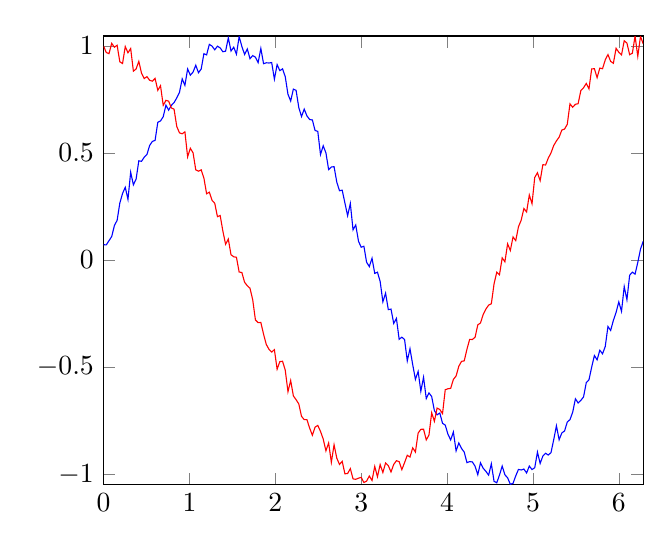
\begin{tikzpicture}
   \begin{axis}[
      domain=0:6.2832,samples=200,
      legend style={
         overlay,
         at={(-0.5,0.5)},
         anchor=center},
      every axis plot post/.append style={mark=none},
      enlargelimits=false]

   \addplot {sin(deg(x)+3)+rand*0.05};
   \addplot {cos(deg(x)+2)+rand*0.05};
   \legend{Signal 1,Signal 2}
   \end{axis}
\end{tikzpicture}
\end{document}
